\documentclass{beamer}
\usepackage{graphicx}
\usepackage{paralist}
\usepackage{outlines}

\title{Filters, Blending Modes, Guide Lines, Importing Images, and Contact Sheets.}
\author{Joshua Paul Barnard}
\titlegraphic{\vspace{-10mm}\includegraphics[width = .8\textwidth]{images/photoshop.jpg}} 
\date{\vspace{-5em}} 


\mode <presentation>
\usetheme{Warsaw}
\usecolortheme{default}

\setbeamerfont{footline}{size=\fontsize{5}{8}\selectfont}

\definecolor{darkred}{rgb}{20,0,0}
\definecolor{darkgreen}{RGB}{40,110,20}
\definecolor{darkpurple}{RGB}{30,0,30}
\definecolor{chardonnay}{RGB}{255, 255, 204}

\setbeamercolor*{palette primary}{fg=white, bg=darkgreen}


\begin{document}
	{
		\setbeamertemplate{footline}{} 
		\setbeamertemplate{headline}{} 
		\begin{frame}
			\vspace{-35pt}
			\maketitle
		\end{frame}
	}

	\section{}	
\subsection{Table of Contents - Week 4}
\begin{frame}
	\frametitle{Table of Contents - Week 4}
	\begin{columns}
		\column{.6\textwidth}
		\vspace{-25pt}
		\begin{itemize}
			\item Announcements
			\item Filters
			\item Blending Modes
			\item Crop Tool \& Importing Images
			\item Guide Lines \& Workspace
			\item Making Contact Sheets
		\end{itemize}
		\column{.45\textwidth}
		\includegraphics[width=.85\textwidth]{images/ps.jpg}
	\end{columns}
\end{frame}

\begin{frame}
	\frametitle{Announcement - Syllabus Update}
	\begin{outline}
		\1 Changes to the Syllabus with the Grading System.
		\1 Participation and Discussions have been unchanged.
		\1 Exercises was renamed to Assignments, and total percent of grade changed from 25\% to 20\%.
		\1 Projects was added
		\2 A Midterm Portfolio Project was added, worth 10\% of your overall grade.
		\2 The Final Presentation Project's total percent of grade changed from 30\% to 15\%.
		\1 Examination's total percent of grade changed from 30\% to 35\%.
		\2 Weekly Quizzes were added, worth a total 10\% of your grade.
		\2 The Midterm Exam's total percent of grade changed from 15\% to 10\%.
		\2 The Final Exam is unchanged.
	\end{outline}
\end{frame}

\begin{frame}
	\frametitle{Announcements - Course Outline Update}
		\begin{columns}
		\column{.5\textwidth}
		\vspace{-25pt}
	\begin{center}
				\begin{itemize}
			\item Updated Syllabus
		\end{itemize}
	\includegraphics[width = 1.0\textwidth]{images/syllabus update.png}
\end{center}
		\column{.5\textwidth}

		\begin{center}
							\begin{itemize}
				\item Updated Course Outline
			\end{itemize}
			\includegraphics[width = 1.1\textwidth]{images/Outline Update.png}
		\end{center}
	\end{columns}

\end{frame}

\begin{frame}
	\frametitle{Announcements - Schedule}
	\begin{outline}
		\1 We need more time in lab to complete assignments and projects.
		\1 Lectures will be moved online
		\2 Released the first day of each week (Monday)
		\1 It is important to watch the lectures before coming to lab!
		\2 A quiz will be due before the first day of each week (Sunday at midnight)
	\end{outline}
\begin{center}
				\includegraphics[width = 0.9\textwidth]{images/schedule.png}
\end{center}
\end{frame}

\begin{frame}
	\frametitle{Announcements - Discussions}
	\begin{outline}
		\1 Discussions for each week will now consist of two parts
		\2 Part 1 will consist of reading articles or watching videos, and commenting to the class anything you found interesting, or about anything you did not understand.
		\2 Part 2 will consist of choosing a topic from a list, researching the topic, and writing about what you learned to your fellow classmates.
		\1 You must reply to two of your classmates posts by either answering their questions, expanding upon their ideas, or adding something to the discussion (not just "I agree", etc)
		\1 You must use proper spelling and grammar, write in complete sentences, and have a minimum of 100 words.
	\end{outline}
\end{frame}

\begin{frame}
	\frametitle{Announcements - Adobe Bridge}
	\begin{outline}
		\1 We will be coming back to Adobe Bridge in Week 13 for Adobe Camera Raw and Lightroom
		\1 If you want to use Adobe Bridge, please go ahead and download it and begin using it.
		\2 https://www.adobe.com/products/bridge.html
		\1 Just let me know if you have any questions about using Bridge.
	\end{outline}
\begin{center}
	\includegraphics[width = 0.65\textwidth]{images/what-is-adobe-bridge-cc.jpg}
\end{center}
\end{frame}


	\section{Filters}
		\begin{frame}
		\frametitle{Filters}
		\begin{center}
			\includegraphics[width = 0.8\textwidth]{images/66821-20100927_fg01.jpg}
		\end{center}
	\end{frame}
	
			\subsection{What are Filters?}		
	\begin{frame}
		\frametitle{What are Filters?}
	\begin{outline}
		\1 You can use filters to clean up or retouch your photos, apply special art effects that give your image the appearance of a sketch or an impressionistic painting, or even create unique transformations using distortions and lighting effects. 
		\1 Filters are applied to the active, visible layer or a selection.
		\1 All filters can be applied to 8‑bit images, but not all filters work with 16-bit and 32-bit images.
	\end{outline}
\begin{center}
	\includegraphics[width=.7\textwidth]{images/filters.png}
	\end{center}
		\end{frame}

\begin{frame}
		\frametitle{Performance}

	\begin{outline}
		\1 Some filters are processed entirely in RAM. If you don’t have enough available RAM to process a filter effect, you may get an error message.
		\1 You can free up extra RAM by closing background programs.
		\1 You can also manually change the RAM usage, along with other memory related settings:
		\2 From the Menu Bar:  Edit - Preferences - Performance
	\end{outline}
\begin{center}
	\includegraphics[width=.7\textwidth]{images/performance.png}
	\end{center}
\end{frame}


\subsection{How to use Filters}	
\begin{frame}
	\frametitle{How to use Filters}
	\begin{outline}
		\1 Select a layer
		\1 Go to the menu bar
		\2 Select Filter
		\2 Then choose a filter
		\1 Be careful, the filter will be applied directly to the layer and will permanently alter it.  
	\end{outline}
	\begin{center}
		\includegraphics[width = 0.75\textwidth]{images/apply filter.png}
	\end{center}
\end{frame}

\subsection{Smart Filters}	
\begin{frame}
	\frametitle{What are Smart Filters?}
	\begin{outline}
		\1 Smart Filters are stored as layer effects in the Layers panel and can be readjusted at any time, working from the original image data contained in the Smart Object.
		\1 They are non-destructive.
		\2 You can simply hide or remove their effects from your layer.
		\1 They give you more control and you can even stack filters ontop of each other.
	\end{outline}
	\begin{center}
		\includegraphics[width = 0.85\textwidth]{images/smart filters.png}
	\end{center}
\end{frame}

\begin{frame}
	\frametitle{Filter Gallery}
	\begin{outline}
		\1 To access the Filter Gallery, navigat to the Menu Bar:
		\2 Click Filter
		\2 Then Filter Gallery
	\end{outline}
	\begin{center}
		\includegraphics[width = 1.0\textwidth]{images/get to filter gallery.png}
	\end{center}
\end{frame}
	
	
	\section{Blending Modes}
	\begin{frame}
		\frametitle{Blending Modes}
		\begin{center}
			\includegraphics[width = 0.55\textwidth]{images/blending modes 2.jpg}
		\end{center}
	\end{frame}
	
\subsection{What are Blending Modes?}
\begin{frame}
	\frametitle{What are Blending Modes?}
	\begin{outline}
		\1 The blending mode specified in the options bar controls how pixels in the image are affected by a painting or editing tool. 
		\1 Think of the following colors when applying a blending mode:
		\2 The base color is the original color in the image.
		\2 The blend color is the color being applied with the painting or editing tool.
		\2 The result color is the color resulting from the blend.
	\end{outline}
	\begin{center}
		\includegraphics[width = 0.7\textwidth]{images/Photoshop-blend-layer-effects-orange-1.jpg}
	\end{center}
\end{frame}

\subsection{How to Apply Blending Modes}
\begin{frame}
	\frametitle{How to Apply Blending Modes}
	\begin{outline}
		\1 The Blending Modes are in the Layers Panel.
		\1 It is the drop-down menu next to Opacity
	\end{outline}
	\begin{center}
	\includegraphics[width = 1.0\textwidth]{images/blending modes 3.png}
\end{center}
\end{frame}


\subsection{Blending Modes Descriptions}
\begin{frame}
	\frametitle{Normal}
	\begin{outline}
		\1 Normal:
		\2 Edits or paints each pixel to make it the result color. This is the default mode. (Normal mode is called Threshold when you’re working with a bitmapped or indexed-color image.)
		\1 Dissolve: 
		\2 Edits or paints each pixel to make it the result color. However, the result color is a random replacement of the pixels with the base color or the blend color, depending on the opacity at any pixel location.
	\end{outline}
\end{frame}

\begin{frame}
	\frametitle{Darken}
	\begin{outline}
		\1 Darken:
		\2 Looks at the color information in each channel and selects the base or blend color—whichever is darker—as the result color. Pixels lighter than the blend color are replaced, and pixels darker than the blend color do not change.
		\1 Multiply:  
		\2 Looks at the color information in each channel and multiplies the base color by the blend color. The result color is always a darker color. Multiplying any color with black produces black. Multiplying any color with white leaves the color unchanged. When you’re painting with a color other than black or white, successive strokes with a painting tool produce progressively darker colors. The effect is similar to drawing on the image with multiple marking pens.
	\end{outline}
\end{frame}

\begin{frame}
	\frametitle{Darken (part 2)}
	\begin{outline}
		\1 Color Burn:
		\2 Looks at the color information in each channel and darkens the base color to reflect the blend color by increasing the contrast between the two. Blending with white produces no change.
		\1 Linear Burn:
		\2 Looks at the color information in each channel and darkens the base color to reflect the blend color by decreasing the brightness. Blending with white produces no change.
		\1 Darker Color:  
		\2 Compares the total of all channel values for the blend and base color and displays the lower value color. Darker Color does not produce a third color, which can result from the Darken blend, because it chooses the lowest channel values from both the base and the blend color to create the result color.
	\end{outline}
\end{frame}

\begin{frame}
	\frametitle{Lighten}
	\begin{outline}
		\1 Lighten:
		\2 Looks at the color information in each channel and selects the base or blend color—whichever is lighter—as the result color. Pixels darker than the blend color are replaced, and pixels lighter than the blend color do not change.
		\1 Screen:
		\2 Looks at each channel’s color information and multiplies the inverse of the blend and base colors. The result color is always a lighter color. Screening with black leaves the color unchanged. Screening with white produces white. The effect is similar to projecting multiple photographic slides on top of each other.
		\1 Color Dodge:
		\2 Looks at the color information in each channel and brightens the base color to reflect the blend color by decreasing contrast between the two. Blending with black produces no change.
	\end{outline}
\end{frame}

\begin{frame}
	\frametitle{Lighten (part 2)}
	\begin{outline}
		\1 Linear Dodge (Add)
		\2 Looks at the color information in each channel and brightens the base color to reflect the blend color by increasing the brightness. Blending with black produces no change.
		\1 Lighter Color
		\2 Compares the total of all channel values for the blend and base color and displays the higher value color. Lighter Color does not produce a third color, which can result from the Lighten blend, because it chooses the highest channel values from both the base and blend color to create the result color.
	\end{outline}
\end{frame}

\begin{frame}
	\frametitle{Overlay}
	\begin{outline}
		\1 Overlay:
		\2 Multiplies or screens the colors, depending on the base color. Patterns or colors overlay the existing pixels while preserving the highlights and shadows of the base color. The base color is not replaced, but mixed with the blend color to reflect the lightness or darkness of the original color.
		\1 Soft Light:
		\2 Darkens or lightens the colors, depending on the blend color. The effect is similar to shining a diffused spotlight on the image. If the blend color (light source) is lighter than 50\% gray, the image is lightened as if it were dodged. If the blend color is darker than 50\% gray, the image is darkened as if it were burned in. Painting with pure black or white produces a distinctly darker or lighter area, but does not result in pure black or white.
	\end{outline}
\end{frame}

\begin{frame}
	\frametitle{Overlay (part 2)}
	\begin{outline}
		\1 Hard Light:
		\2 Multiplies or screens the colors, depending on the blend color. The effect is similar to shining a harsh spotlight on the image. If the blend color (light source) is lighter than 50\% gray, the image is lightened, as if it were screened. This is useful for adding highlights to an image. If the blend color is darker than 50\% gray, the image is darkened, as if it were multiplied. This is useful for adding shadows to an image. Painting with pure black or white results in pure black or white.
		\1 Vivid Light
		\2 Burns or dodges the colors by increasing or decreasing the contrast, depending on the blend color. If the blend color (light source) is lighter than 50\% gray, the image is lightened by decreasing the contrast. If the blend color is darker than 50\% gray, the image is darkened by increasing the contrast.
	\end{outline}
\end{frame}

\begin{frame}
	\frametitle{Overlay (part 3)}
	\begin{outline}
		\1 Linear Light
		\2 Burns or dodges the colors by decreasing or increasing the brightness, depending on the blend color. If the blend color (light source) is lighter than 50\% gray, the image is lightened by increasing the brightness. If the blend color is darker than 50\% gray, the image is darkened by decreasing the brightness.
		\1 Pin Light
		\2 Replaces the colors, depending on the blend color. If the blend color (light source) is lighter than 50\% gray, pixels darker than the blend color are replaced, and pixels lighter than the blend color do not change. If the blend color is darker than 50\% gray, pixels lighter than the blend color are replaced, and pixels darker than the blend color do not change. This is useful for adding special effects to an image.
	\end{outline}
\end{frame}

\begin{frame}
	\frametitle{Overlay (part 4)}
	\begin{outline}
		\1 Hard Mix
		\2 Adds the red, green and blue channel values of the blend color to the RGB values of the base color. If the resulting sum for a channel is 255 or greater, it receives a value of 255; if less than 255, a value of 0. Therefore, all blended pixels have red, green, and blue channel values of either 0 or 255. This changes all pixels to primary additive colors (red, green, or blue), white, or black.
	\end{outline}
\end{frame}

\begin{frame}
	\frametitle{Difference}
	\begin{outline}
		\1 Difference:
		\2 Looks at the color information in each channel and subtracts either the blend color from the base color or the base color from the blend color, depending on which has the greater brightness value. Blending with white inverts the base color values; blending with black produces no change.
		\1 Exclusion:
		\2 Creates an effect similar to but lower in contrast than the Difference mode. Blending with white inverts the base color values. Blending with black produces no change.		\1 Subtract:
		\2 Looks at the color information in each channel and subtracts the blend color from the base color. In 8- and 16-bit images, any resulting negative values are clipped to zero.
		\1 Divide:  
		\2 Looks at the color information in each channel and divides the blend color from the base color.
	\end{outline}
\end{frame}

\begin{frame}
	\frametitle{Color / Hue}
	\begin{outline}
		\1 Hue:  
		\2 Creates a result color with the luminance and saturation of the base color and the hue of the blend color.
		\1 Saturation:  
		\2 Creates a result color with the luminance and hue of the base color and the saturation of the blend color. Painting with this mode in an area with no (0) saturation (gray) causes no change.		
		\1 Color
		\2 Creates a result color with the luminance of the base color and the hue and saturation of the blend color. This preserves the gray levels in the image and is useful for coloring monochrome images and for tinting color images.
		\1 Luminosity
		\2 Creates a result color with the hue and saturation of the base color and the luminance of the blend color. This mode creates the inverse effect of Color mode.
	\end{outline}
\end{frame}

	\section{Crop Tool \& Importing Images}
		\begin{frame}
		\frametitle{Crop Tool \& Importing Images}
		\begin{center}
			\includegraphics[width = 1.0\textwidth]{images/crop-tool-photoshop-2020.jpg}
		\end{center}
	\end{frame}
	
		\subsection{Importing Images}
\begin{frame}
	\frametitle{Importing an Image to a New Project}
	\begin{itemize}
		\item Select the image in windows file explorer.
		\item Drag the image into Photoshop, next to your active tab.
	\end{itemize}
	\begin{center}
		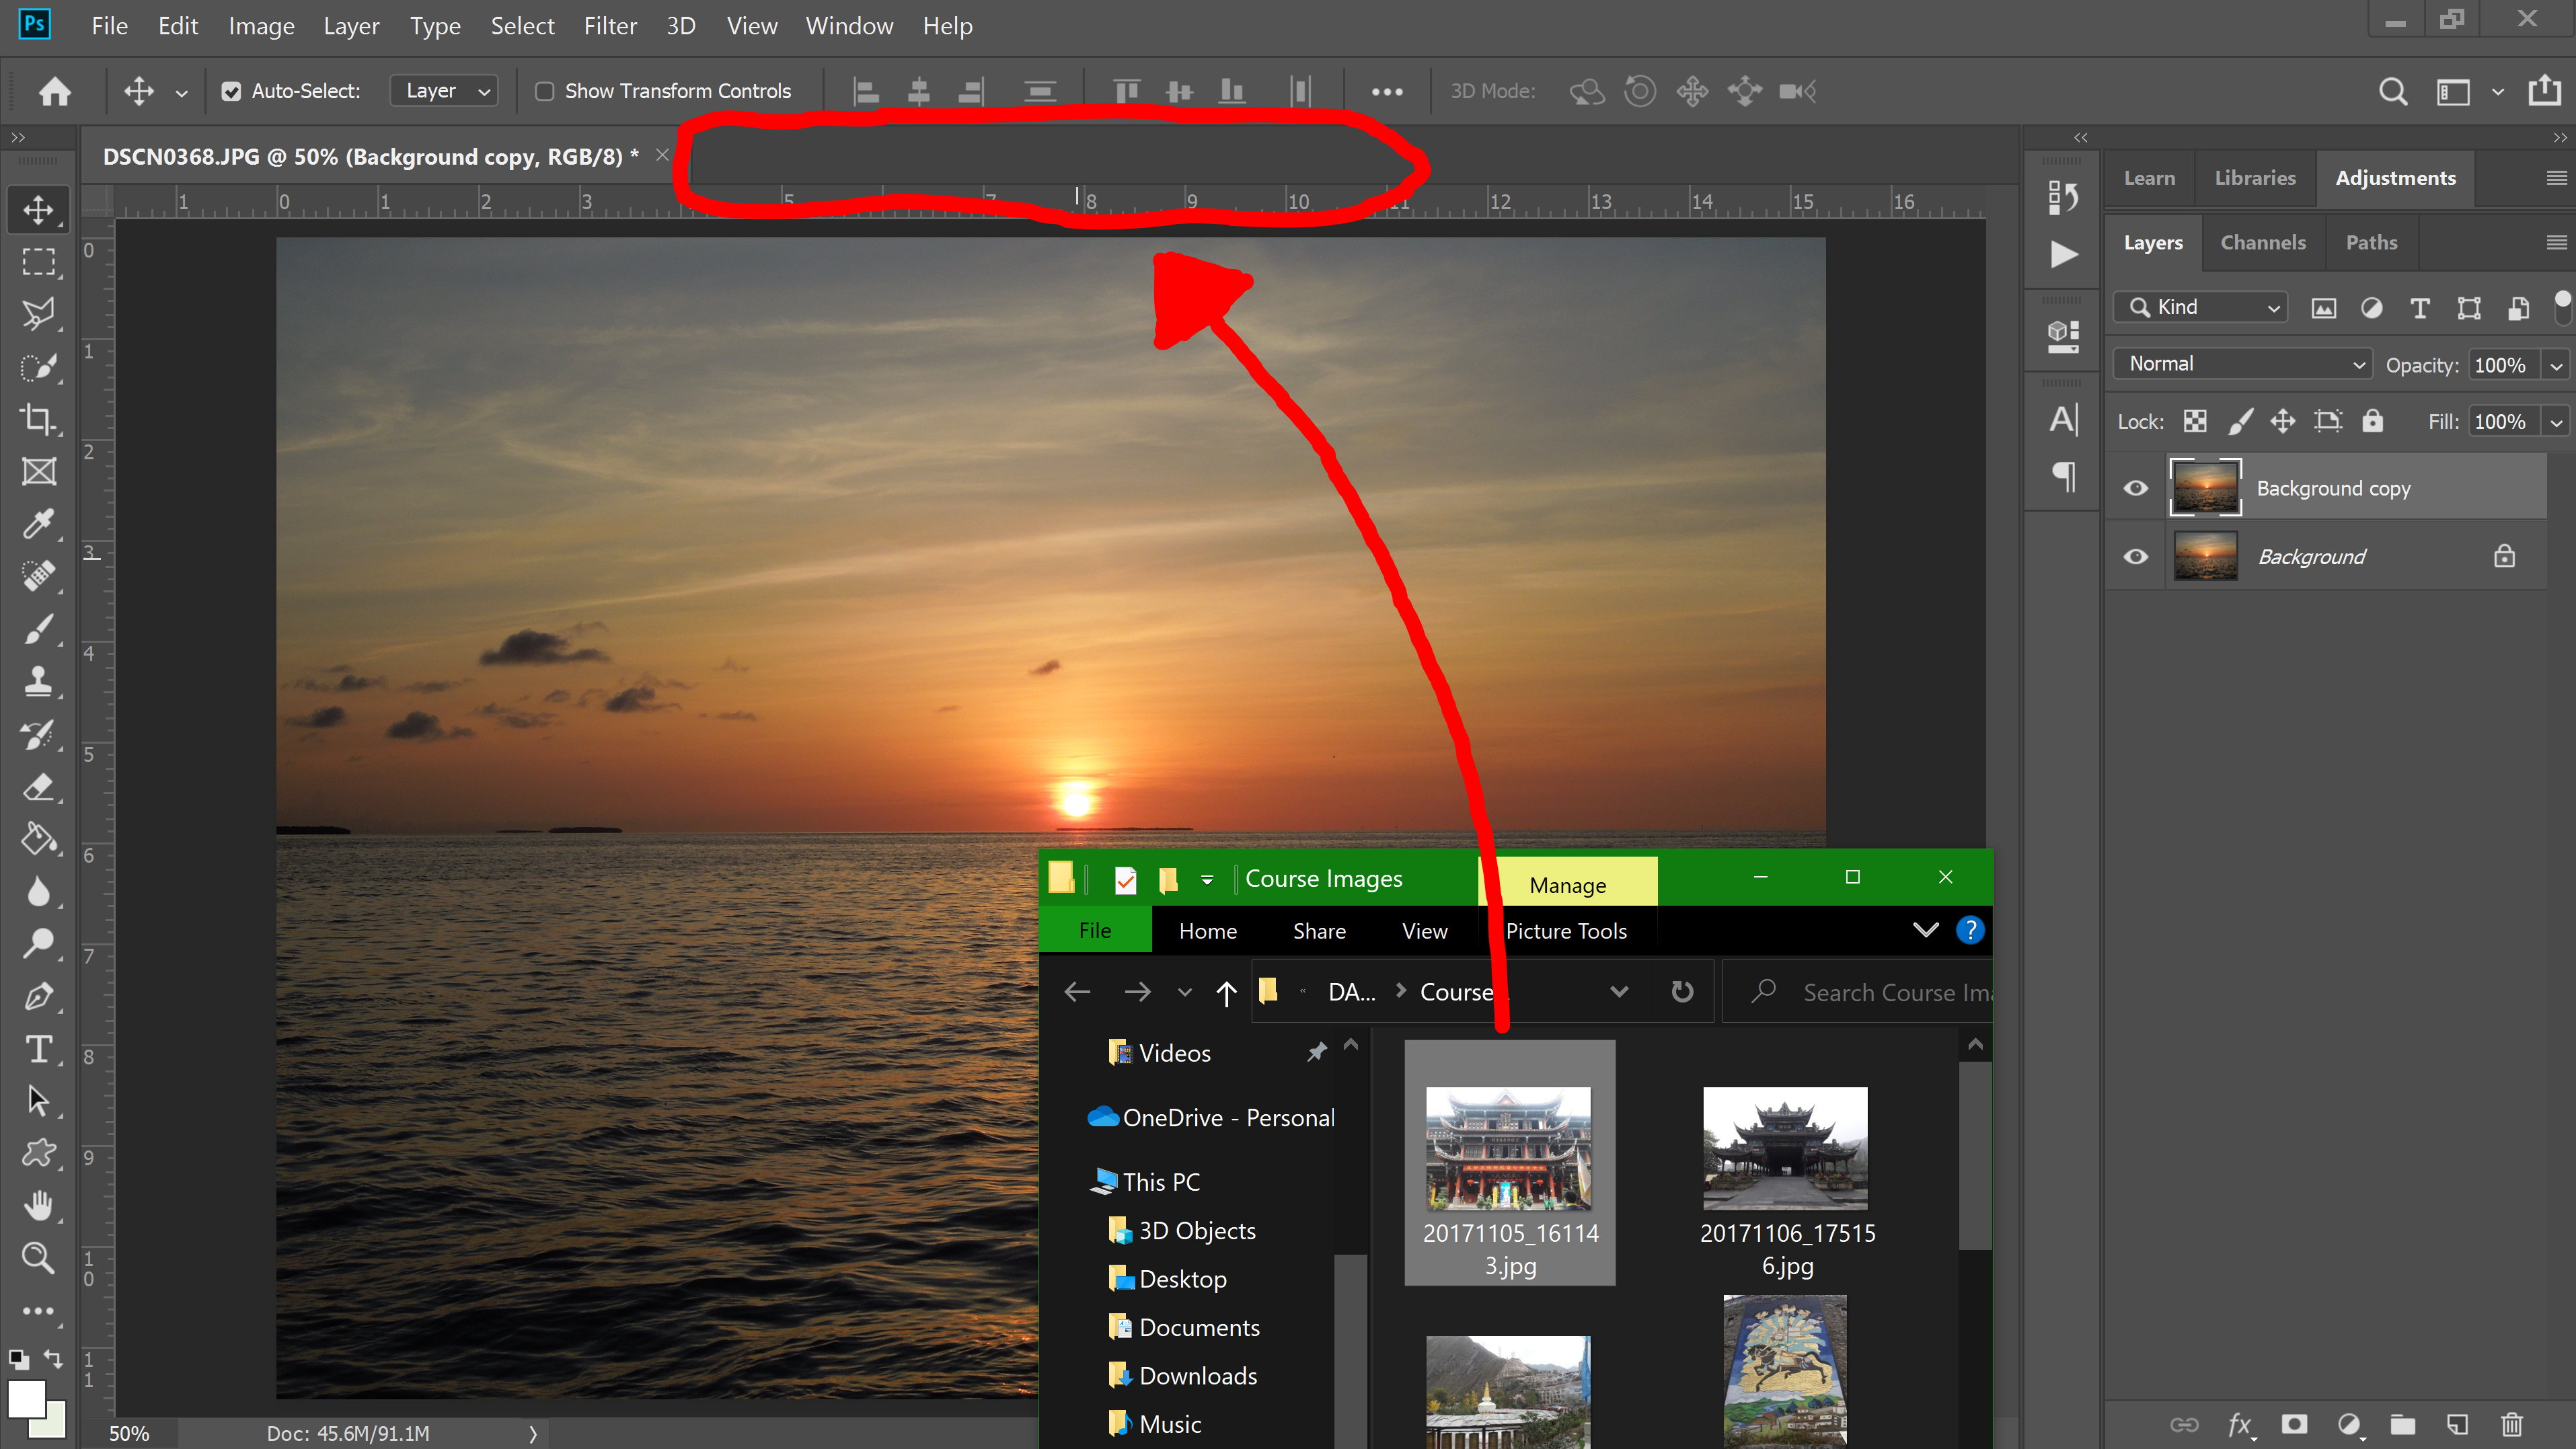
\includegraphics[width = 1.0\textwidth]{images/import 1.png}
	\end{center}
\end{frame}

\begin{frame}
	\frametitle{Importing an Image to an Existing Project}
	\begin{outline}
		\1 Select the image in windows file explorer.
		\1 Drag the image into the active Photoshop image.
		\1 You will then crop the image you are importing.
		\1 The image will be imported as a new layer.
	\end{outline}
	\begin{center}
		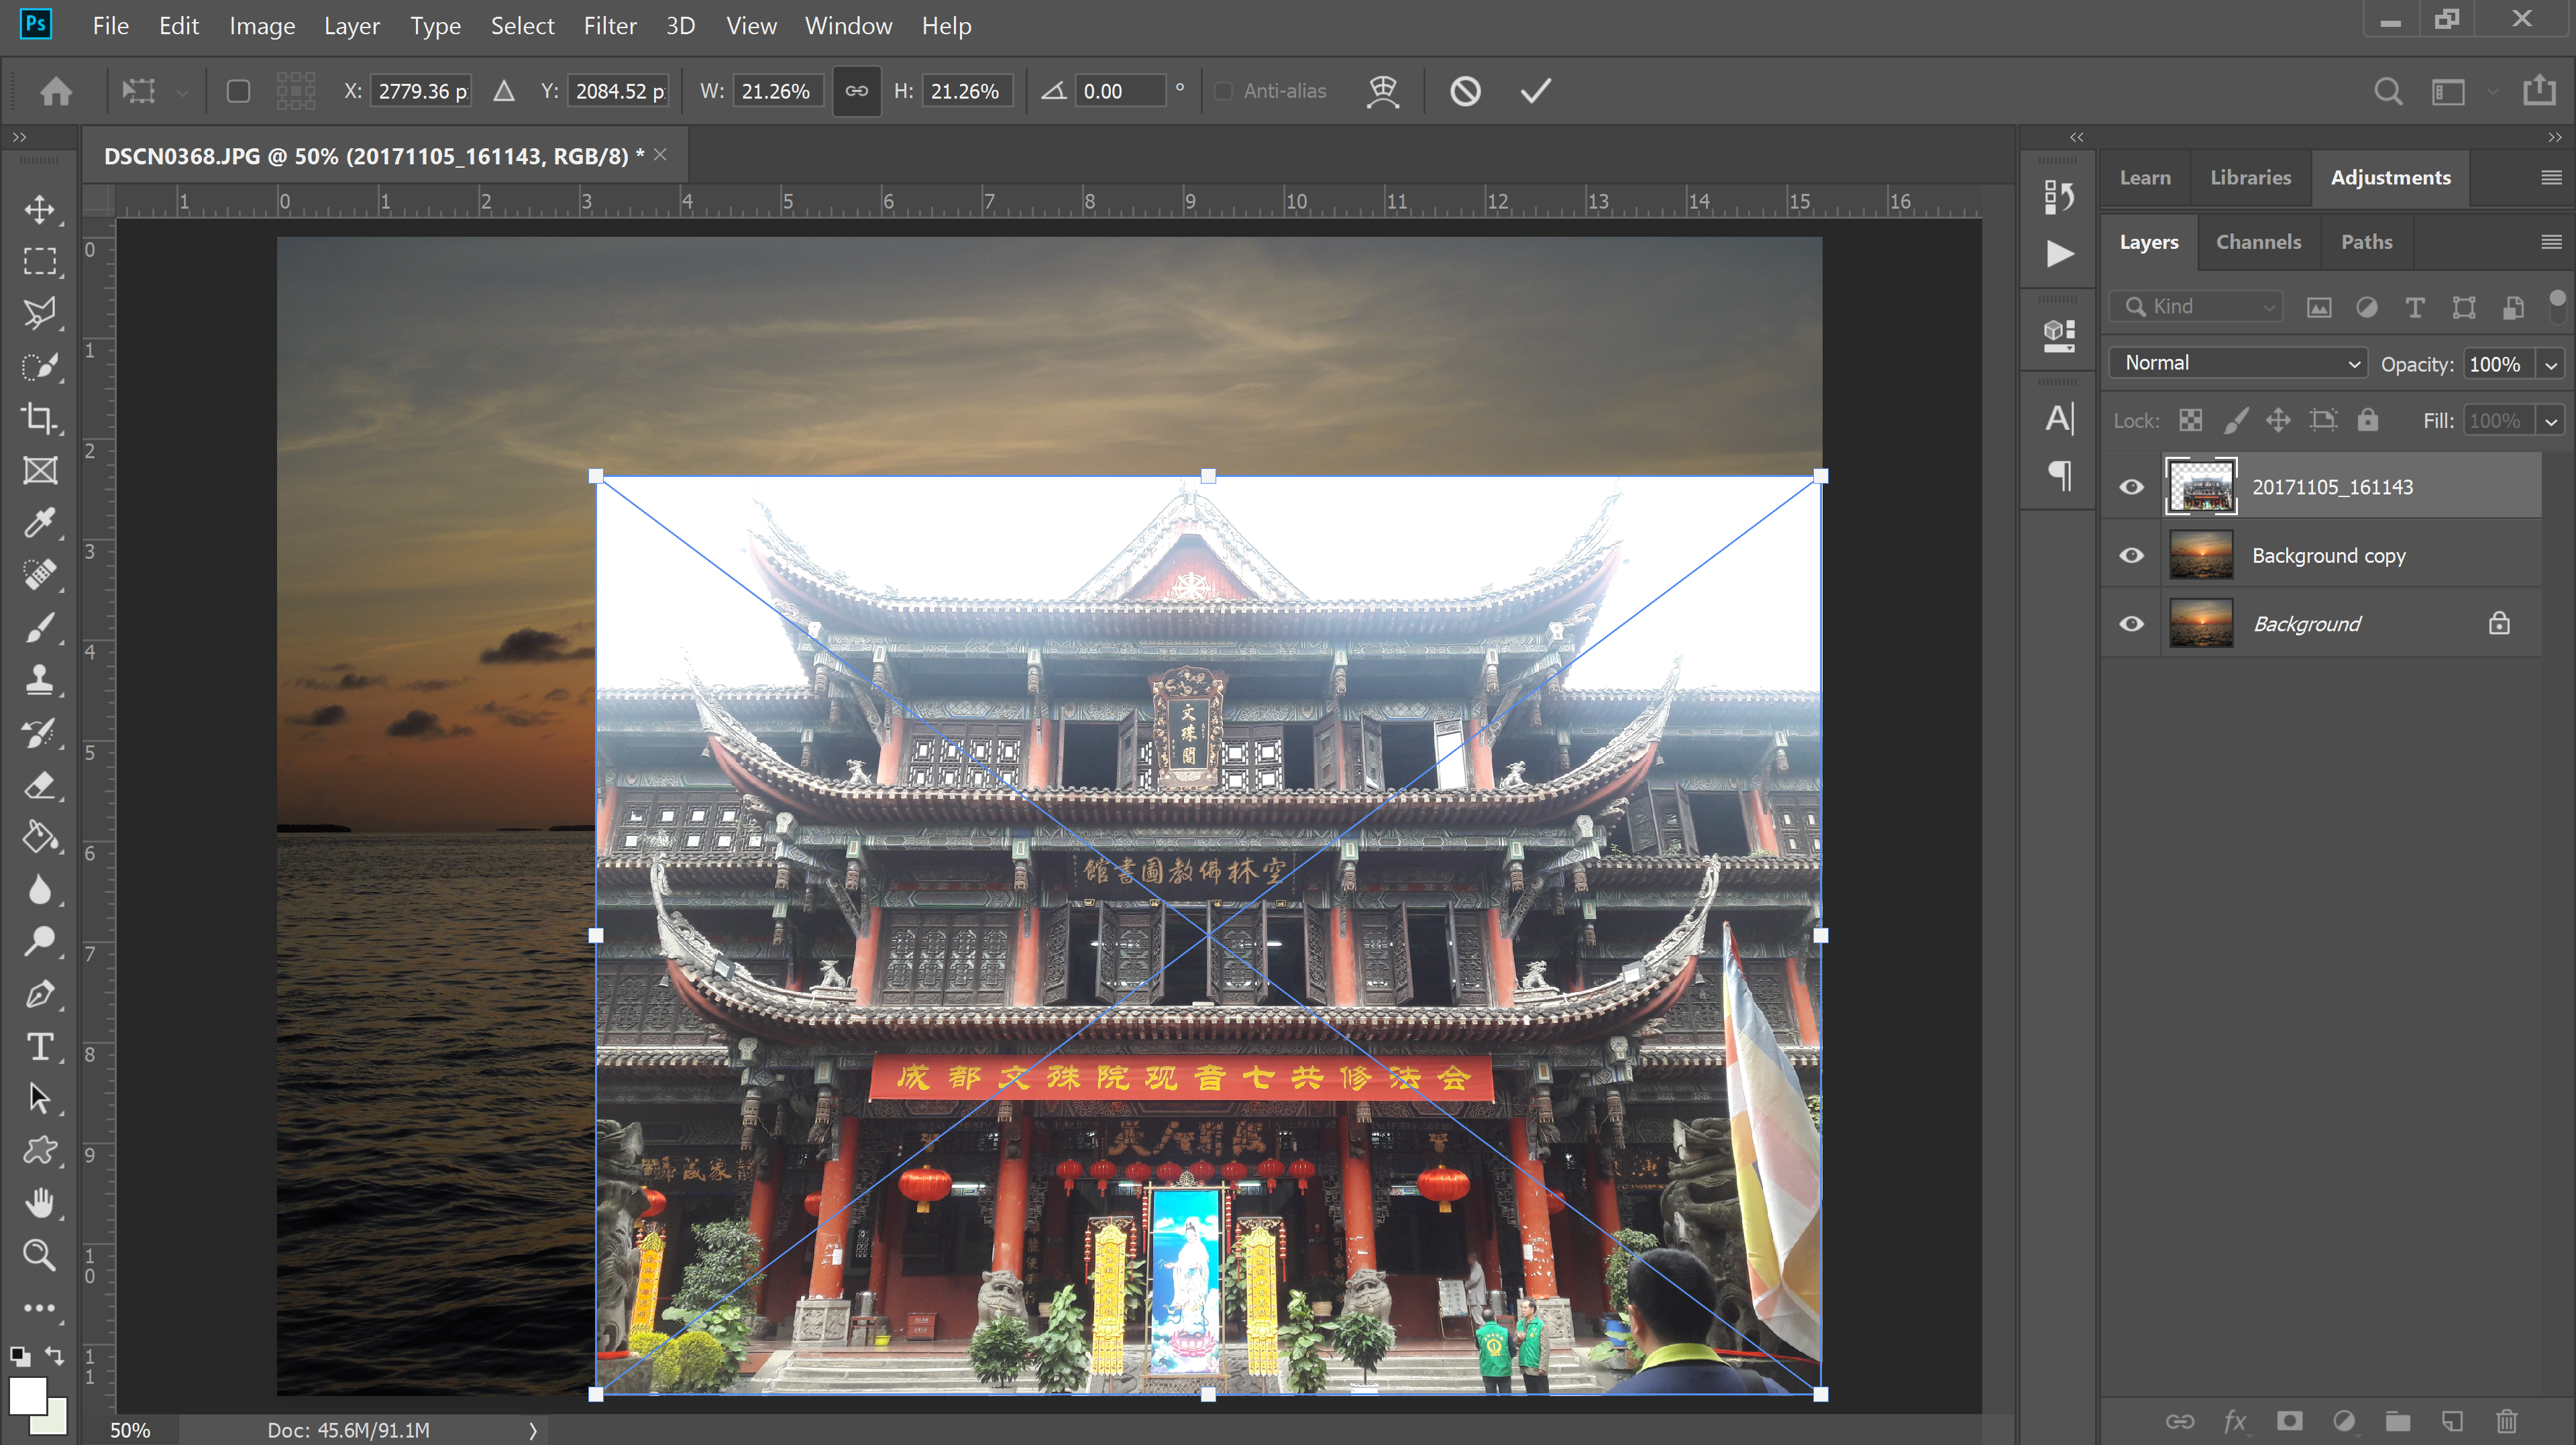
\includegraphics[width = 0.75\textwidth]{images/import 2.png}
	\end{center}
\end{frame}

		\subsection{Crop Tool}
\begin{frame}
	\frametitle{The Crop Tool}
	\begin{itemize}
		\item Cropping is the process of removing portions of a photo to create focus or strengthen the composition. 
		\item Use the Crop tool to crop and straighten photos in Photoshop. 
		\item The Crop tool is non-destructive, and you can choose to retain the cropped pixels to optimize the crop boundaries later.
		\item The Crop tool also provides intuitive methods to straighten a photo while cropping.
	\end{itemize}
	\begin{center}
		\includegraphics[width = 0.75\textwidth]{images/crop 1.png}
	\end{center}
\end{frame}

\begin{frame}
	\frametitle{Crop Options}
	\begin{outline}
		\1 Size and proportions:
		\2 Choose a ratio or size for the crop box. You can also choose a preset, enter your own, or even define your own preset values for later use.
		\1 Overlay Options:
		\2 Choose a view to display overlay guides while cropping. Guides such as Rule of Thirds, Grid, and Golden Ratio are available. To cycle through all the options, press O.
	\end{outline}
	\begin{center}
		\includegraphics[width = 1.0\textwidth]{images/crop 2.png}
	\end{center}
\end{frame}

\begin{frame}
	\frametitle{Crop Options (part 2)}
	\begin{outline}
		\1 Show Cropped Area:
		\2 Enable this option to display the area that is cropped. If this option is disabled, only the final area is previewed.
		\1 Enable Crop Shield:
		\2 Use the crop shield to overlay the cropped areas with a tint. You can specify a color and opacity. If you Enable Auto Adjust Opacity, the opacity is reduced when you edit the crop boundaries.
		\1 Delete cropped pixels
		\2 Disable this option to apply a non-destructive crop and retain pixels outside the crop boundaries. Non-destructive cropping does not remove any pixels. You can later click the image to see areas outside current crop borders.
		\2 Enable this option to delete any pixels that are outside the crop area. These pixels are lost and are not available for future adjustments.
	\end{outline}
\end{frame}

\subsection{Perspective Crop Tool}
\begin{frame}
	\frametitle{Perspective Crop Tool}
	\begin{outline}
		\1 Crop your images and fix perspective distortions at the same time.
		\1 Unlike Photoshop's standard Crop Tool, the Perspective Crop Tool does not automatically place a cropping border around the image. So the first thing we need to do is draw one ourselves. 
		\2 To do that, I'll click in the top left corner of the photo and, with my mouse button held down, I'll drag diagonally downward to the bottom right corner:
		\1 Line up the perspective grid with the edges of your subject
	\end{outline}
	\begin{center}
		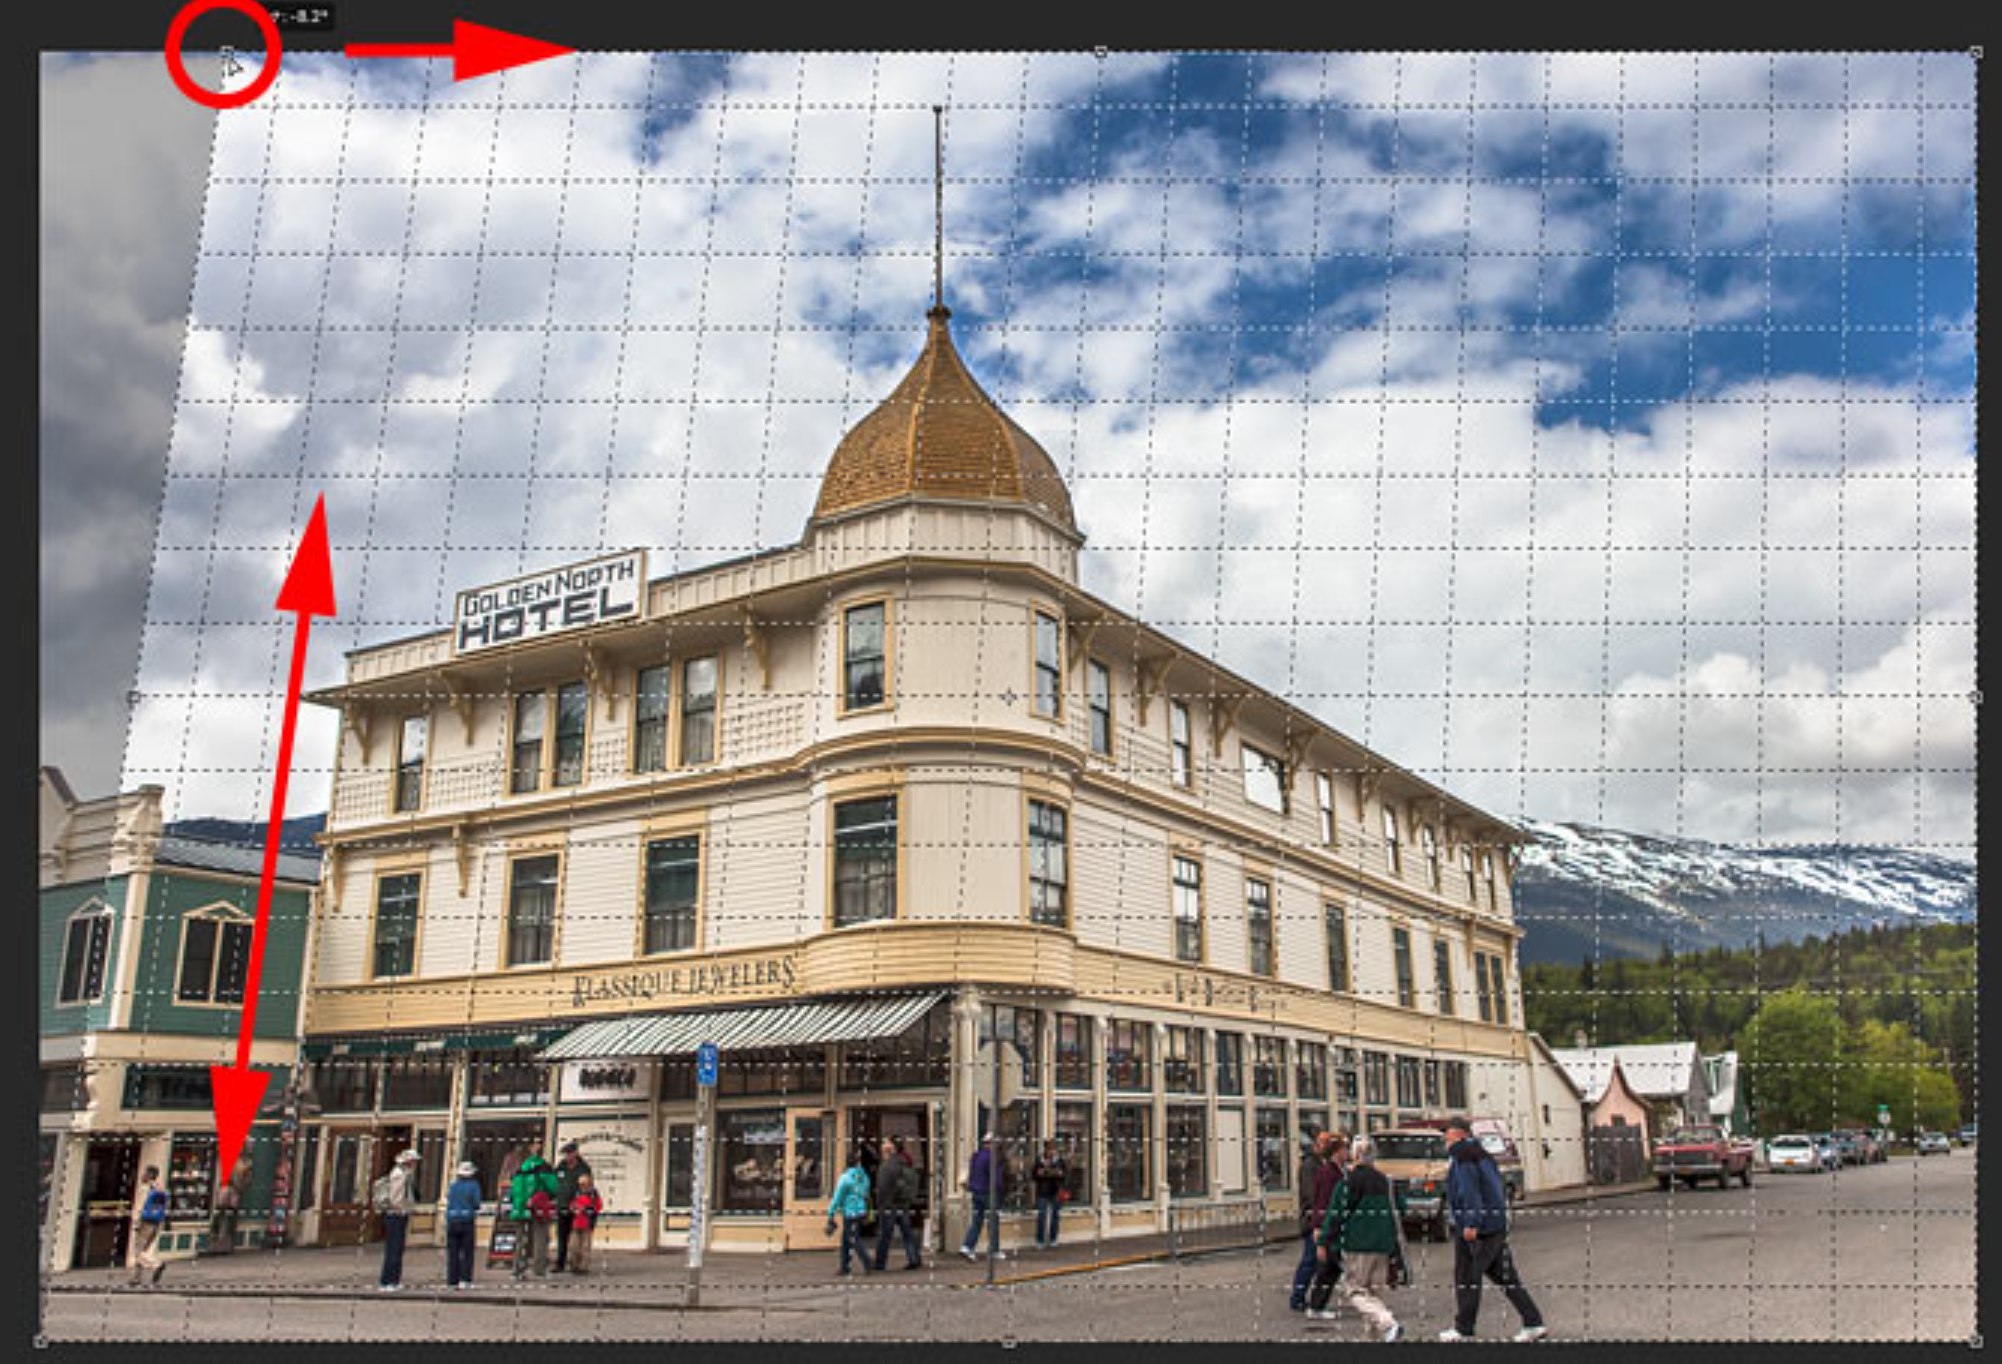
\includegraphics[width = 0.4\textwidth]{images/crop 3.png}
	\end{center}
\end{frame}
		
		
	\section{Guide Lines \& Workspace}
		\begin{frame}
		\frametitle{Guide Lines, Rulers \& Workspace}
		\begin{center}
			\includegraphics[width = 0.8\textwidth]{images/smart guides and rulers.jpg}
		\end{center}
	\end{frame}
	
	\subsection{What are Guide Lines?}
	\begin{frame}
		\frametitle{What are Guide Lines?}
		\begin{outline}
			\1 Guides and the grid help in positioning images or elements precisely.
			\1 Guides appear as nonprinting lines that float over the image that can be moved or removed. 
			\2 You can also lock them so that you don’t move them by accident.
			\1 Selections, selection borders, and tools snap to a guide or the grid when dragged within 8 screen (not image) pixels. Guides also snap to the grid when moved. You can turn this feature on and off.
		\end{outline}
		\begin{center}
			\includegraphics[width = 0.5\textwidth]{images/guide lines.png}
		\end{center}
	\end{frame}
	
	\subsection{How to access Guides?}
	\begin{frame}
		\frametitle{How to access Guides and Grids?}
		\begin{center}
			\includegraphics[width = 0.8\textwidth]{images/guides.png}
		\end{center}
	\end{frame}

	\begin{frame}
	\frametitle{Locking and Moving Guides}
	\begin{outline}
		\1 If you want to lock all guides, choose View - Guides - Lock Guides submenu.
		\1 Select the Move tool
		\2 Position the pointer over the guide (the pointer turns into a double-headed arrow).
		\2 Drag the guide to move it.
	\end{outline}
\end{frame}

	\subsection{Ruler}
	\begin{frame}
	\frametitle{Ruler}
	\begin{outline}
		\1 When visible, rulers appear along the top and left side of the active window. 
		\1 Markers in the ruler display the pointer’s position when you move it.
		\1 Changing the ruler origin (the 0, 0 mark on the top and left rulers) lets you measure from a specific point on the image.
		\1 The ruler origin also determines the grid’s point of origin.
		\1 Use the View menu to show or hide the rulers, the grid, or the guide.
		\1 To enable/disable the ruler:
		\2 Menu Bar:  View - Ruler
		\2 or press Ctrl + R on the keyboard.
	\end{outline}
\end{frame}



	\begin{frame}
	\frametitle{Creating Guides from Ruler}
	\begin{outline}
		\1 Drag from the vertical ruler to create a horizontal guide.
		\1 Drag from the horizontal ruler to create a vertical guide.
	\end{outline}
		\begin{center}
	\includegraphics[width = 0.5\textwidth]{images/guides 2.png}
\end{center}
\end{frame}

\subsection{Snap/Snap to}
	\begin{frame}
	\frametitle{Snap/Snap to}
			\begin{columns}
		\column{0.5\textwidth}
		\vspace{-25pt}
		\begin{center}
	\begin{itemize}
		\item You can change what you are working with will snap to
		\item Go to the menu bar, then in the View menu.
		\item Hold down Ctrl while working to prevent snapping.
	\end{itemize}
\end{center}
\column{.5\textwidth}
	\begin{center}
			\includegraphics[width = 1.0\textwidth]{images/snap.png}
	\end{center}
\end{columns}
\end{frame}



\subsection{Workspace}
	\begin{frame}
	\frametitle{How to Duplicate Layers}
	\begin{outline}
		\1 Select Layer in panel.
		\1 Right click
		\1 Select Duplicate Layer
		\1 Name the new layer
	\end{outline}
	\begin{center}
		\includegraphics[width = 0.5\textwidth]{images/duplicate.png}
	\end{center}
\end{frame}

	\begin{frame}
	\frametitle{Arrange Projects in Photoshop}
	\begin{outline}
		\1 You can show multiple photoshop projects at once
		\1 In the Menu Bar, select Window - Arrange
		\1 Use "Tile Vertically" to split each project.
		\1 Use "Consolidate All to Tabs" to return to a single project.
	\end{outline}
	\begin{center}
		\includegraphics[width = 0.75\textwidth]{images/arrange.png}
	\end{center}
\end{frame}

	\begin{frame}
	\frametitle{How to transfer layers between projects}
	\begin{outline}
		\1 Have both projects open at the same time.
		\1 use Tile Vertically to re-arrange the windows.
		\1 Go to the project with the layer you want to transfer.
		\1 Select the layer.
		\1 Drag that layer to the other window
	\end{outline}
	\begin{center}
		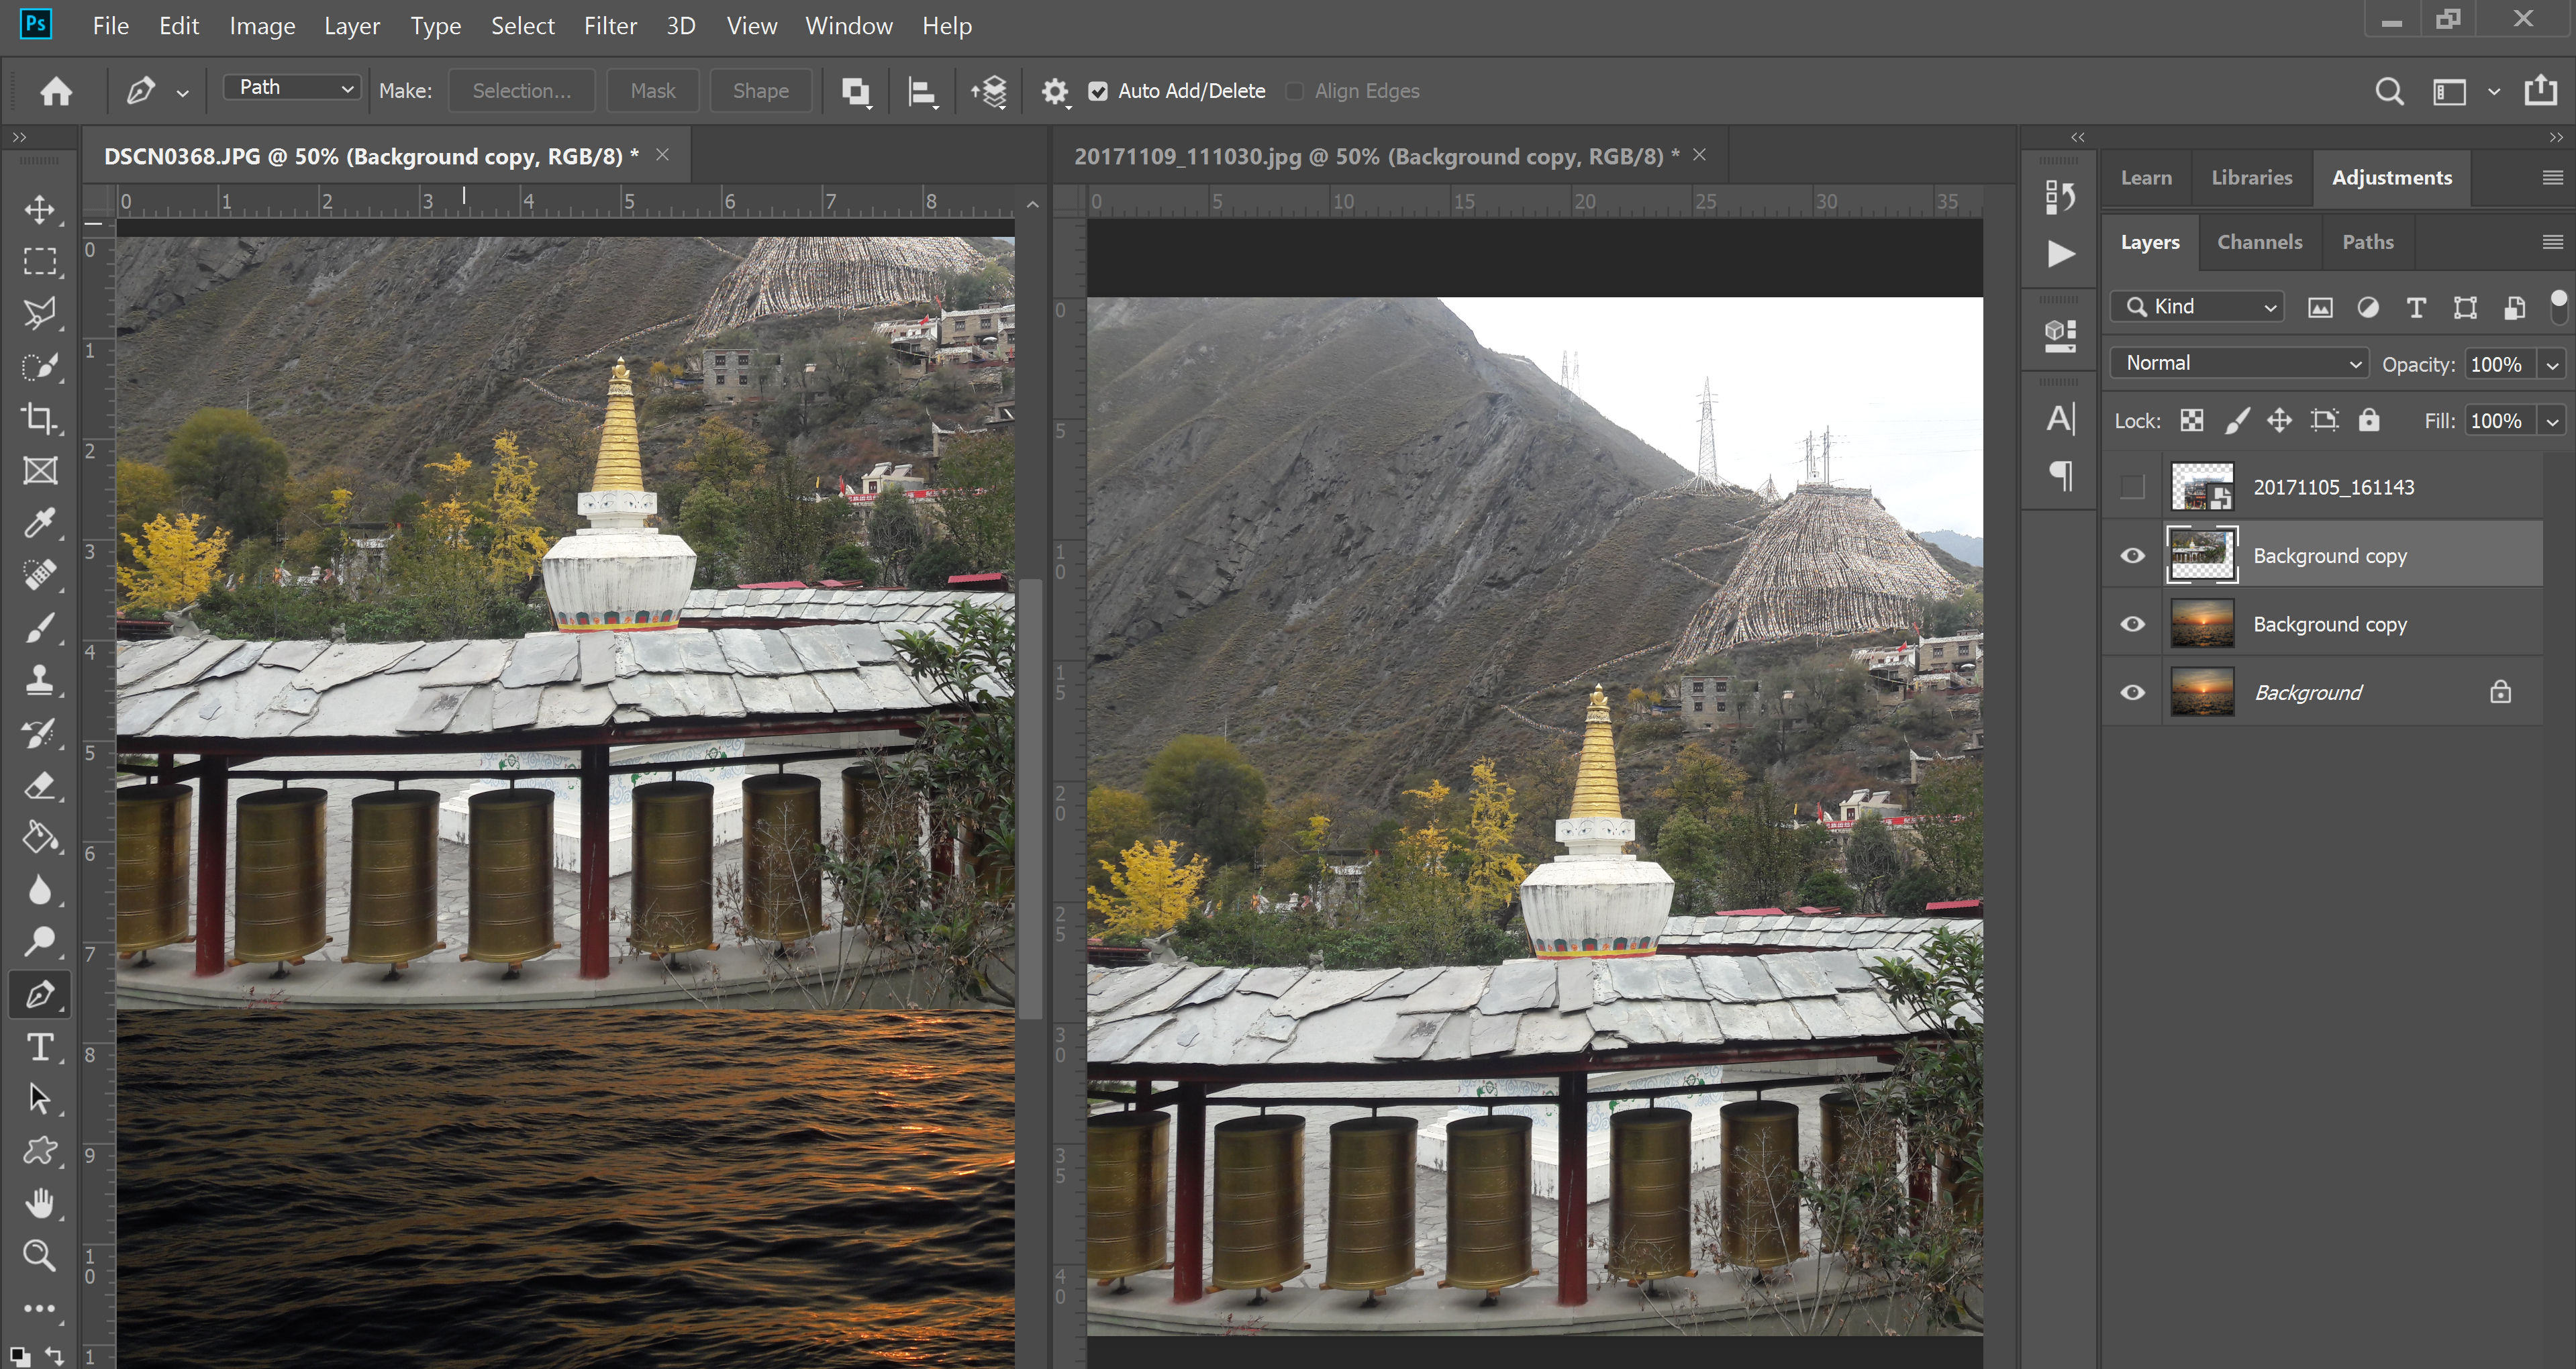
\includegraphics[width = 0.75\textwidth]{images/transfering layers.png}
	\end{center}
\end{frame}



	\section{Contact Sheets}	
		\begin{frame}
		\frametitle{Contact Sheets}
		\begin{center}
			\includegraphics[width = 1.0\textwidth]{images/contact.jpg}
		\end{center}
	\end{frame}
	
	\subsection{How to make a contact sheet}
	\begin{frame}
		\frametitle{How to make a contact sheet}
		\begin{columns}
	\column{.5\textwidth}
	\vspace{-25pt}
	\begin{itemize}
		\item Menu Bar:  File - Automate - Contact Sheet II...
	\end{itemize}
	\column{.75\textwidth}
	\includegraphics[width=.85\textwidth]{images/contact2.jpg}
\end{columns}
	\end{frame}

	\begin{frame}
	\frametitle{How to make a contact sheet}
	\begin{columns}
		\column{.5\textwidth}
		\vspace{-25pt}
		\begin{itemize}
			\item You are able to choose individual files, an entire folder, or all of the currently open documents in photoshop.  
			\item Make sure to setup the correct number of rows and columns for your contact sheets.  
		\end{itemize}
		\column{.75\textwidth}
		\includegraphics[width=.85\textwidth]{images/contact3.jpg}
	\end{columns}
\end{frame}

	\section{}	
		\subsection{End Card}
	\begin{frame}
		\frametitle{End Card}	
		\begin{columns}
			\column{.6\textwidth}
			\vspace{-25pt}
			\begin{itemize}
				\item Joshua Paul Barnard
				\item Computer Science Instructor
				\item Mendocino College
			\end{itemize}
			\begin{itemize}
				\item This Presentation was made in \LaTeX
				\item For the Fall 2022 semester.  
			\end{itemize}
			\begin{itemize}
				\item jbarnard@mendocino.edu
				\item github.com/JoshuaPaulBarnard
			\end{itemize}
			\column{.45\textwidth}
			\includegraphics[width=.85\textwidth]{images/shone farm wine pouring - vert.png}
		\end{columns}
	\end{frame}
	
\end{document}